\section{Optimal predictor}

The quality of prediction can be quantified through the Mean Square Prediction Error, defined as:
\[\text{MSPE}=\mathbb{E}\left[ {\left(y(t+k)-\hat{y}(t+k\mid t) \right)}^2 \right]\]

\paragraph*{Minimization}
Our goal is to minimize the squares of prediction errors. 
The prediction depends on past samples through a function:
\[\hat{y}(t+k\mid t)=f(y(t),y(t-1),\dots)\]
Therefore, we would need to minimize all suitable functions for prediction and select the best one, which is generally impractical due to the vast number of possible functions. 
However, by constraining ourselves to linear predictors, this task becomes more manageable.

Linear predictors take the form:
\[\hat{y}(t+k\mid t)=\alpha_0y(t)+\alpha_1y(t-1)+\dots=\sum_{i=0}^{+\infty}\alpha_i y(t-i)\]
Here, $\alpha_i \in \mathbb{R}$ such that $\sum_{i=0}^{+\infty}\alpha_i<+\infty$. 
We can express this general formulation using operatorial representation as:
\[\hat{y}(t+k\mid t)=\left(\alpha_0+\alpha_1z^{-1}\alpha_2z^{-2}+\dots\right)y(t)=F_{\alpha}(z)y(t)\]
We assume that $\hat{y}(t+k\mid t)$ is the steady-state output of a linear digital filter with transfer function $F_{\alpha}(z)$.

\subsection{Optimal predictor design}
We aim to determine the optimal coefficients $\alpha_0^{\circ},\alpha_1^{\circ},\alpha_2^{\circ},\dots$ of the linear predictor:
\[\hat{y}(t+k\mid t,\alpha)=\sum_{i=0}^{+\infty}\alpha_i y(t-i)\]
such that the mean squared prediction error is minimized:
\[\min_{\alpha_0,\alpha_1,\alpha_2,\dots}\mathbb{E}\left[{\left( y(t+k)-\hat{y}(t+k\mid t,\alpha) \right)}^2\right] \]

We begin by considering a generic Moving Average process:
\[y(t)=W(z)e(t) =\sum_{i=0}^{+\infty}w_i e(t-i) \qquad e(t)\sim WN(0,\lambda^2)\]
When we perform a time shift, we have:
\[y(t-1)=\sum_{i=0}^{+\infty}w_i e(t-1-i)\]
We can then insert this expression into the predictor, resulting in:
\begin{align*}
    \hat{y}(t+k\mid t)  &=\alpha_0\sum_{i=0}^{+\infty}w_i e(t-i)+\alpha_1\sum_{i=0}^{+\infty}w_i e(t-1-i)+\dots \\
                    &=\beta_0e(t)+\beta_1e(t-1)+\dots \\
                    &=\sum_{i=0}^{+\infty}\beta_i e(t-1)
\end{align*}
where the factor $\beta$ is found by grouping all elements referring to the same time instant.

We can reformulate the optimization problem with respect to $\alpha$ as a new optimization problem with respect to $\beta$. 
This can be expressed as:
\[\min_{\beta_0,\beta_1,\beta_2,\dots}\mathbb{E}\left[{\left( y(t+k)-\hat{y}(t+k\mid t,\beta) \right)}^2\right]\]

Considering that $y(t+k)$ admits the Moving Average representation, we write:
\[y(t+k)=\sum_{i=0}^{+\infty}w_i e(t+k-i)=\underbrace{\sum_{j=0}^{k-1}w_j e(t+k-j)}_{\text{future } e(t)} +\underbrace{\sum_{i=0}^{+\infty}w_{k+i}e(t-i)}_{\text{past and present } e(t)} \]

We can express the prediction error as follows:
\begin{align*}
    \mathbb{E}\left[ {\left(\varepsilon(t+k\mid t)\right)}^2 \right]  &= \mathbb{E}\left[ {\left(\sum_{i=0}^{k-1}w_j e(t+k-i)+\sum_{i=0}^{+\infty}w_{k+i}e(t-i)-\sum_{i=0}^{+\infty}\beta_i e(t-1)\right)}^2 \right] \\
                                                                &= \mathbb{E}\left[ {\left(\sum_{i=0}^{k-1}w_j e(t+k-i)+\sum_{i=0}^{+\infty}w_{k+i}e(t-i)-\beta_i e(t-1)\right)}^2 \right] 
\end{align*}
Expanding the square, we have:
\begin{multline*}
    \mathbb{E}\left[ {\left(\varepsilon(t+k\mid t)\right)}^2 \right] = \mathbb{E}\left[ \underbrace{{\left(\sum_{i=0}^{k-1}w_j e(t+k-i)\right)}^2}_{\beta \text{ independent}}\right]  +\mathbb{E}\left[\underbrace{{\left(\sum_{i=0}^{+\infty}w_{k+i}e(t-i)-\beta_i e(t-1)\right)}^2}_{\beta \text{ dependent}}\right]  +\\ +2\mathbb{E}\left[\underbrace{\left(\sum_{i=0}^{k-1}w_j e(t+k-i)\sum_{i=0}^{+\infty}w_{k+i}e(t-i)-\beta_i e(t-1)\right)}_0 \right]                       
\end{multline*}
The first term cannot be minimized since there will always be some error in predicting future samples, while the second term depends on $\beta$, requiring minimization to solve the optimization problem:
\[\sum_{i=0}^{+\infty}\beta_i e(t-i)=\sum_{i=0}^{+\infty}w_{k+i}e(t-i)\]

Thus, an optimal predictor satisfies:
\[\beta_i^\circ=w_{k+i} \qquad i=0,1,2,\dots\]
This is termed the optimal predictor from the  White Noise, and its expression is:
\[\hat{y}^\circ=\sum_{i=0}^{+\infty}w_{k+i}e(t-i)\]

\paragraph*{Operatorial representation}
The operatorial representation of a process is:
\[W(z)=\dfrac{C(z)}{A(z)}=w_0+w_1z^{-1}+\dots\]
By performing long division between $C(z)$ and $A(z)$, we obtain:
\[\dfrac{C(z)}{A(z)}=E(z)+\dfrac{z^{-k}F(z)}{A(z)}\]
Here, $k$ is the number of steps in the long division.
This equation is termed the Diophantine equation, useful for rewriting the process at a specific time lag $k$ as:
\begin{align*}
    \hat{y}(t+k\mid t)  &=\dfrac{C(z)}{A(z)}e(t+k) \\
            &=\left[E(z)+\dfrac{z^{-k}F(z)}{A(z)}\right]e(t+k) \\
            &=E(z)e(t+k)+\dfrac{z^{-k}F(z)}{A(z)}e(t+k) \\
            &=E(z)e(t+k)+\dfrac{F(z)}{A(z)}e(t) \\
            &=\underbrace{e_0e(t+k)+e_1e(t+k-1)+\dots+e_{k-1}e(t+1)}_{\text{future } e(t)} +\underbrace{\dfrac{F(z)}{A(z)}e(t)}_{\text{past and present } e(t)} 
\end{align*}
Thus, the optimal predictor in this representation is:
\[\hat{y}(t+k\mid t)=\dfrac{F(z)}{A(z)}e(t)\]
characterized by a finite set of coefficients (those of $F(z)$ and $A(z)$).

\subsection{ White Noise reconstruction}
To practically utilize the optimal predictor we've derived, we require the  White Noise values at each time step. However, obtaining these values directly is often impractical. 
Therefore, we need to reconstruct plausible  White Noise values from the available samples.

The ARMA process under consideration is formulated as:
\[y(t)=W(z)e(t)=\dfrac{C(z)}{A(z)}e(t)\]
Given our assumption that the zeros lie inside the unit circle and that $W(z)$ is asymptotically stable, we can invert the formula to find:
\[e(t)=\dfrac{A(z)}{C(z)}y(t)\]
The transfer function ${W(z)}^{-1}$ is termed the whitening filter.

\paragraph*{Optimal predictor}
Finally, we can express the optimal predictor from data as:
\[\hat{y}(t+k\mid t)=\dfrac{F(z)}{C(z)}y(t)\]

\subsection{Summary}
We summarize our findings as follows:
\begin{itemize}
    \item The optimal predictor, denoted as $\hat{y}(t+k\mid t,s)$, can be expressed as $\dfrac{F(z)}{C(z)}y(t,s)$. 
    \item Due to the presence of roots of $C(z)$ inside the unit circle, $\hat{y}(t+k\mid t)$ represents a stationary stochastic process.
        Thus, we can represent it equivalently as:
        \begin{itemize}
            \item $\hat{y}(t+k\mid t)=\dfrac{F(z)}{C(z)}y(t)$. 
            \item $\hat{y}(t+k\mid t-k)=\dfrac{F(z)}{C(z)}y(t-k)$. 
        \end{itemize}
\end{itemize}

\subsection{Optimal prediction error}
The optimal prediction error is defined as:
\[\varepsilon(t+k\mid t)=E(z)e(t+k)\]
Alternatively, it can be expressed as:
\[\varepsilon(t\mid t-k)=E(z)e(t)\]
This equivalence holds because the prediction error is also a stationary stochastic process, specifically an MA($-1$).

\paragraph*{Variance function}
In the optimal scenario, the variance of the prediction error is given by:
\[\text{Var}\left[\varepsilon(t+k\mid t)\right]=\left(w_0^2+w_1^2+\dots+w_{k-1}^2\right)\lambda^2\]
Since we're dealing with a stationary stochastic process, the variance must converge to a specific value, namely the steady-state variance of the process.
\begin{figure}[H]
    \centering
    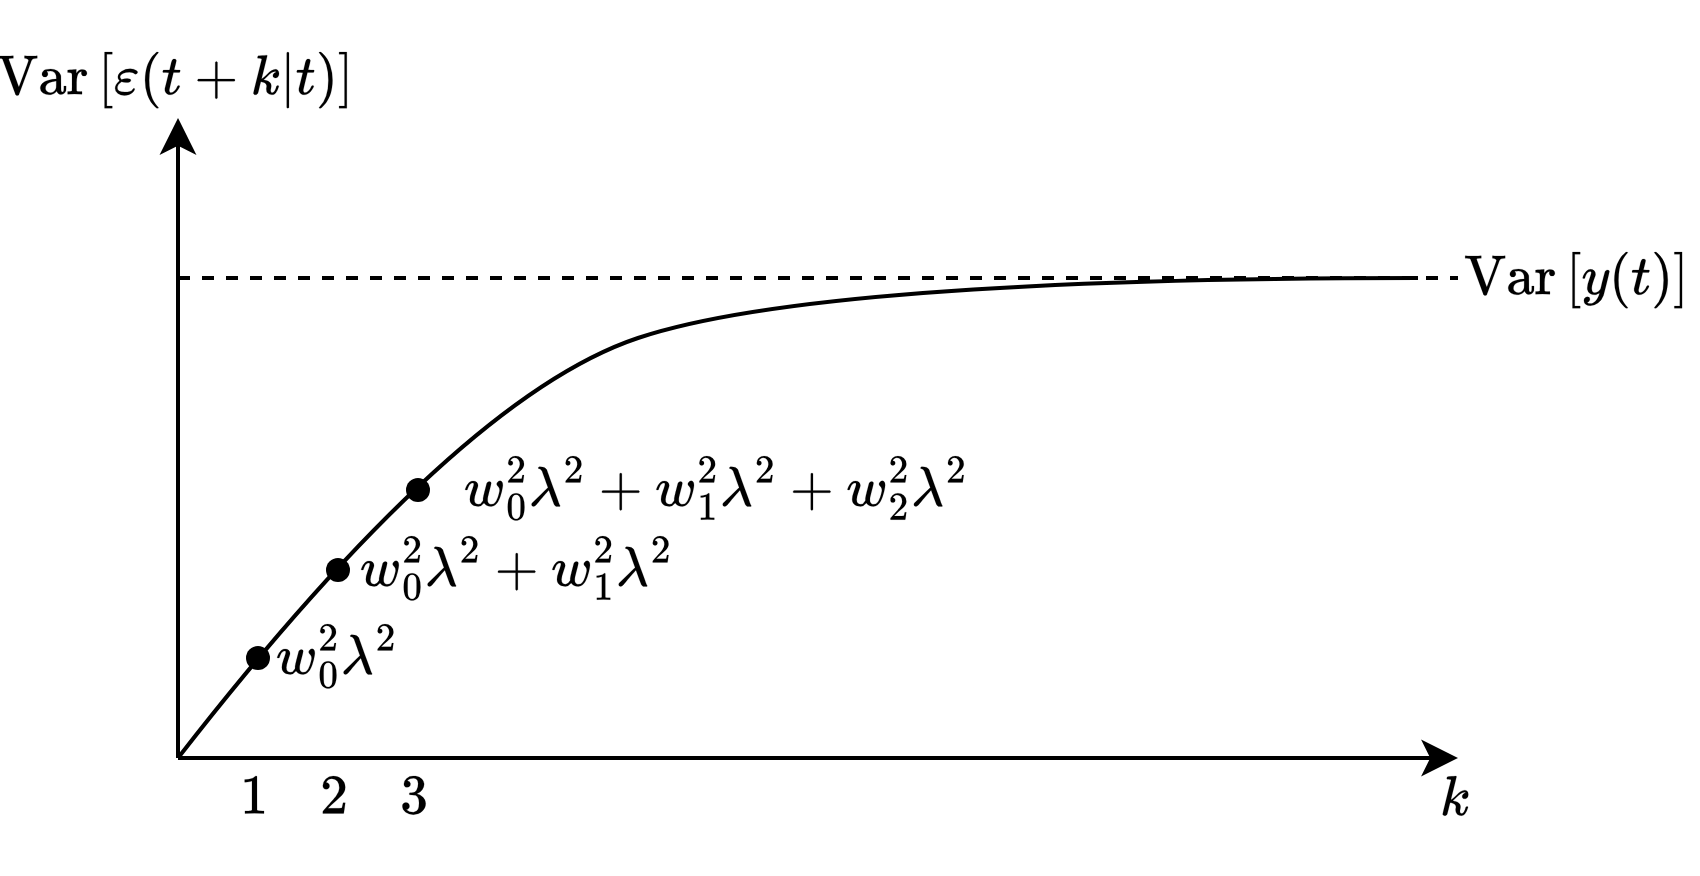
\includegraphics[width=0.75\linewidth]{images/var.png}
    \caption{Variance of the optimal predictor}
\end{figure}
Generally, the following inequality holds:
\[\text{Var}\left[e(t)\right] \leq \text{Var}\left[\varepsilon(t+k\mid t)\right] < \text{Var}\left[y(t)\right]\]